\chapter{Monte Carlo radiation transport technique}
\label{sec:mcrt}
\section{Introduction and Background}
This chapter will provide an overview of the Monte Carlo method and how it is used within the context of \gls{mcrt}. The chapter will then present the details of the MCRT code used as the basis of the subsequent chapters. Validation of this code and details of computational speed up are also presented. Subsequent chapters will expand upon the code for each individual projects needs.

\subsection{Monte Carlo method}\label{sec:mcmethod}
The Monte Carlo method is a numerical analysis technique based upon random numbers, which are used to calculate unknown variables in problems. 

The earliest use of the method is in Buffon's needle experiment of the 18$^{th}$ century~\cite{badger1994lazzarini,beckmann2015history,buffon1785histoire}. Buffon asked the question;

\medskip

``Suppose we have a floor made of parallel strips of wood, each the same width, and we drop a needle onto the floor. What is the probability that the needle will lie across a line between two strips?"

\medskip

The solution to this question is as:
for a needle length \textit{l}, strip separation \textit{s}, and where \textit{x} is the distance from the needle to the closest line. Then using a simple geometrical argument, a needle crosses a strip if $x \leq \tfrac{l}{2} sin \theta$.

$x$ is distributed uniformly in [0, $\tfrac{s}{2}$], and $\theta$ in [0, $\tfrac{\pi}{2}$]. Therefore the probability density function for $x$ is $p(x)=\tfrac{2}{s}$, and $\theta$ is $p(\theta) = \tfrac{2}{\pi}$. The \gls{pdf}, is a function of a variable that gives probability for a variable to a take a given value. The \gls{pdf} is normalised over the whole range of the variable, in this case $x$, and $\theta$.
Thus, as $x$ and $\theta$ are independent variables, giving a joint probability of $p(x,\theta) = \tfrac{4}{s \pi}$.
So the probability of a needle of length l ($l<s$) is:

\begin{equation}
P=\int_0^{\frac{\pi}{2}}\int_0^{\frac{l}{2}sin\theta}\frac{4}{s\pi}dx d\theta = \frac{2 l}{s \pi}\label{eqn:buffon}
\end{equation}


\Cref{eqn:buffon} can be used to carry out a Monte Carlo estimation of pi. A simple rearrangement yields: $\pi = \tfrac{2l}{sP}$ where P is the ratio of needles crossing the line over total number dropped. Laplace was the first to suggest that Buffon's needle experiment could be used to estimate $\pi$~\cite{beckmann2015history}. \Cref{fig:buffon-needle} shows an example of simulation of Buffon's needle experiment.

\begin{figure}[!htb]
\centering
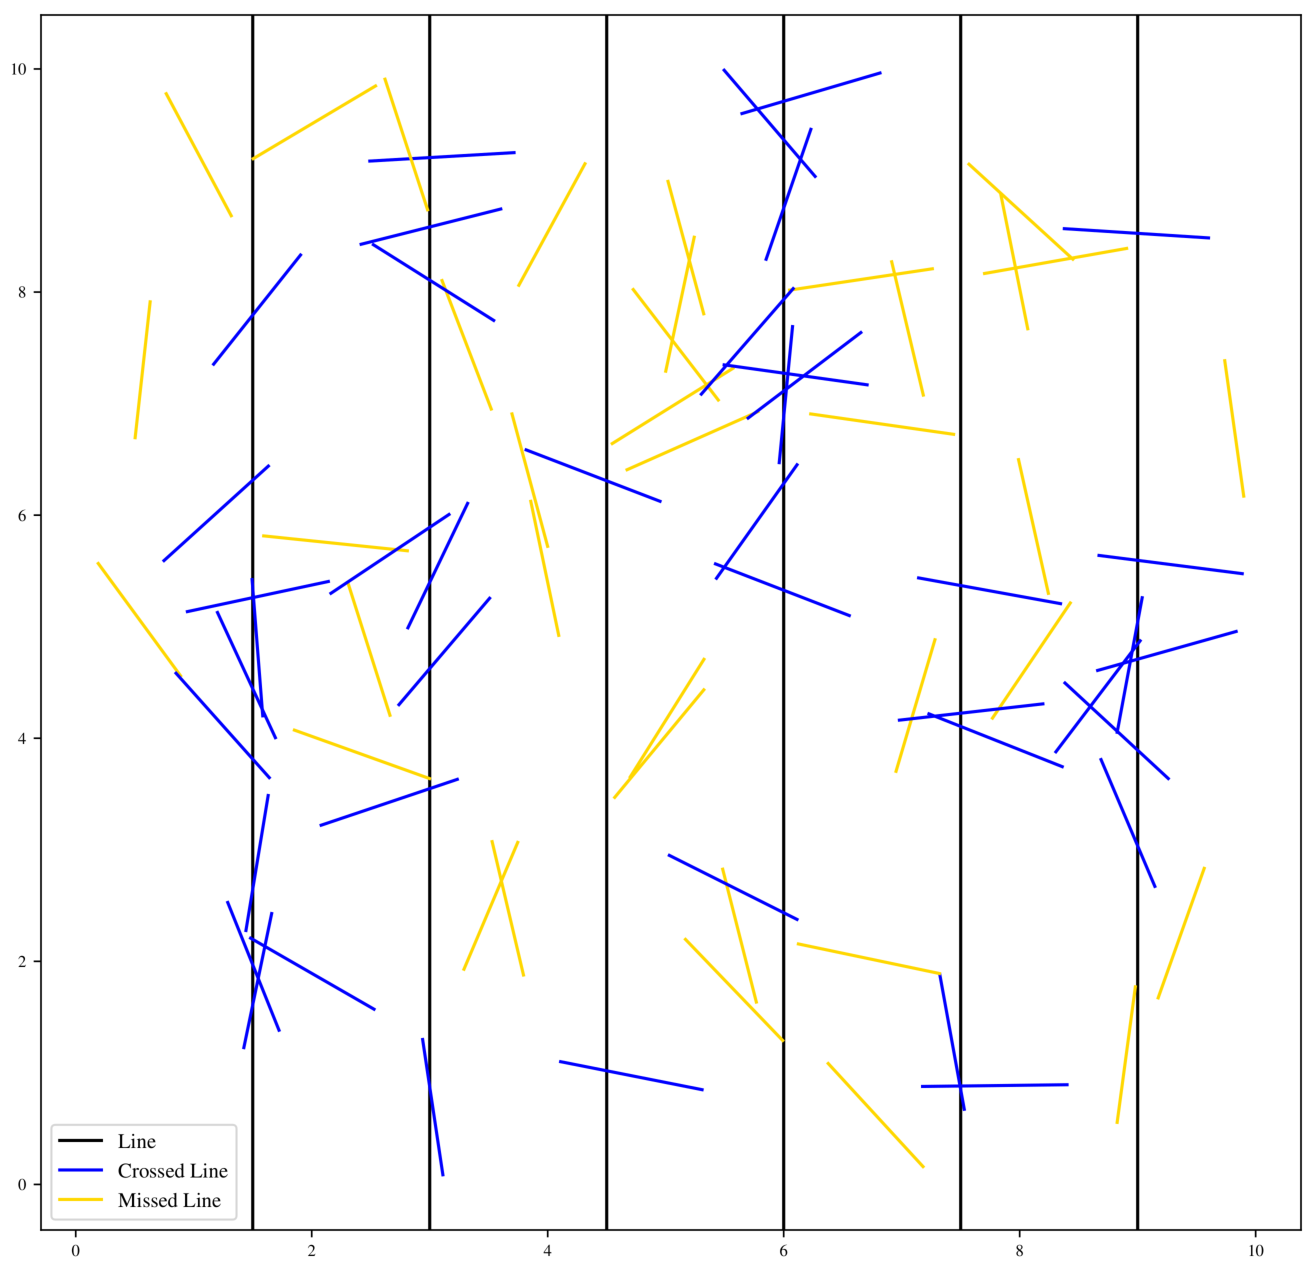
\includegraphics[width=\columnwidth/2]{buffon-pi=317.pdf}
\caption{Sample buffon needle experiment. 100 needles are dropped on a 10 by 10 cm area with lines spaced 1.5cm apart. If a needle lands on a line it is recorded and coloured blue, else it is yellow. This simulation gave a value of pi as 3.17.}
\label{fig:buffon-needle}
\end{figure}

The Monte Carlo method is used in various different disciplines. Ranging from use in the financial sector to analyse investments and stocks by simulating the sources of uncertainty which affect their values~\cite{jackel2002monte,finaceprrof}, use in statistical analysis~\cite{wall2012practical}, and in modern computer generated images (see \cref{fig:ray-trace})~\cite{Kajiyarendering,Cookraytracing}. It is also widely used in astronomy and medicine, in order to simulate the propagation of particles through turbid media. This technique, Monte Carlo radiation transfer, is what makes up the bulk of this thesis and is described in depth in the following sections.

\begin{figure}[!htb]
\centering
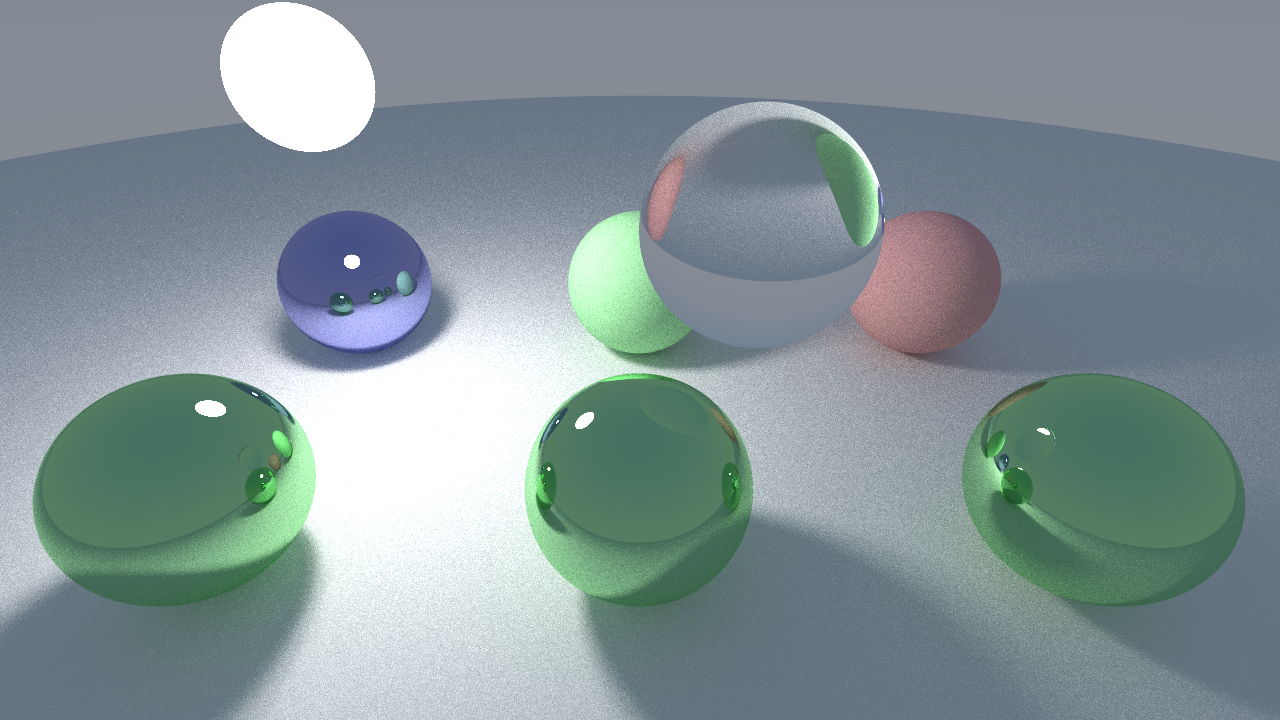
\includegraphics[width=\columnwidth]{ray-tracing.png}
\caption{Computer generated imagery using ray-tracing. Code usd to create image available at: \url{https://github.com/lewisfish/RayTran}}
\label{fig:ray-trace}
\end{figure}
\newpage
\section{Monte Carlo radiation transport algorithm}

\subsection{Introduction \texorpdfstring{$\&$}{and} background}%texorpdfstring supresses warning about pdf bookmarks
The technique that makes up the bulk of this thesis, is the \gls{mcrt} technique. This method was developed at the tail end of the Second World War at the Los Alamos National Laboratory, for the purpose of calculating neutron diffusion though shielding material~\cite{montybeg1,eckhardt1987stan,anderson1986metropolis,ulam1947statistical}. It has since found a myriad of applications from light transport through dusty clouds~\cite{wood1999model}, calculating doses for radiotherapy~\cite{rogers1995beam} to light transport through tissue~\cite{1stmonty}.***more here + link to next section***



\subsubsection{Radiative transfer}
Transport of photons through turbid media, can be modelled analytically using the \gls{rte}. The \gls{rte} models the the radiative losses, and gains by a beam of radiation as it travels through a medium, including: loss of energy due to absorption, loss/gain of energy due to scattering, and energy gain due to emission. Before we derive the \gls{rte}, we first define some terms and physical quantities.


The first term is spectral irradiance, $L_\nu$. Spectral irradiance is defined as the energy flow in a direction \textbf{n}, for a solid angle $d\Omega$, per unit time per unit temporal frequency bandwidth.	
Irradiance is defined as the spectral irradiance over a small frequency range $[\nu, \nu+\Delta \nu]$:

\begin{equation}
	L(\vec{r},\hat{s},t) = L_{\nu}(\vec{r},\hat{s},t)\Delta \nu	
\end{equation}

\noindent Where:

\indent $\vec{r}$ is the position;

\indent $\hat{s}$ is the unit normal vector;

\indent $t$ is the time;

\indent and $L(\vec{r},\hat{s},t)$ is the irradiance [$W \cdot m^{-2}\cdot sr^{-1}$].

\medskip

\begin{figure}[!htb]
	\centering
	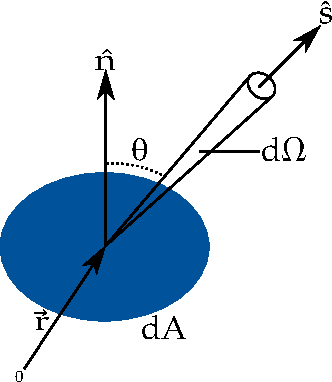
\includegraphics[scale=1.]{diffelement.pdf}
	\caption{Energy flow through area $dA$ within solid angle $d\Omega$ in a direction $\hat{s}$. Adapted from~\cite{wang2012biomedical,chandrasekhar2013radiative}}
	\label{fig:energydiag1}
\end{figure}

The irradiance can be used to determine the energy, $dE$, transported across an area $dA$, in a solid angle $d\Omega$ in a time $dt$ (see~\cref{fig:energydiag1}) is:

\begin{equation}
	dE = L(\vec{r},\hat{s},t) \cdot (\hat{s} \cdot \hat{n})\ dAd\Omega dt
\end{equation}

\noindent Where:

\indent $\hat{n}$ is the unit normal to $dA$;

\indent and $\hat{s}\cdot\hat{n}$ is the angle of the solid angle.

\medskip

Irradiance can also be used to determine the fluence rate, $\phi$, which is defined as the energy flow per unit time, independent of the flow direction.

\begin{equation}
	\phi(\vec{r},t)=\int_{4\pi}L(\vec{r},\hat{s},t)\ d\Omega
\end{equation}

\noindent Where:

\indent $\phi$ is the fluence rate [$W \cdot m^{-2}$].

\medskip

Irradiance is also the main variable in the \gls{rte}, as it describes the light distribution throughout the medium, and by solving the \gls{rte} yields the irradiance, which in turn gives information on the state of the system and all the physical properties of it.

With the irradiance defined, as well as the other quantities that follow, we can now derive the \gls{rte}~\cite{chandrasekhar2013radiative,wang2012biomedical}. We first consider conservation of energy, as shown in~\cref{eqn:enegyconvo}.

\begin{equation}
	dP = -dp_{div} - dp_{ext} + dP_{scatt} + dP_{src}
	\label{eqn:enegyconvo}
\end{equation}

\noindent Where:

\indent $dP$ is the total change in energy in the volume $dAds$ within the solid angle, $d\Omega$, per unit time (see~\cref{fig:energydiag2});

\indent $dP_{div}$ is the energy loss due to the divergence of the radiation beam per unit time;

\indent $dP_{ext}$ is the energy loss due to absorption and scattering within $dAdsd\Omega$;

\indent $dP_{scatt}$ is the energy gain due to scattering from $\hat{s}'$ into $d\Omega$ per unit time;

\indent and $dP_{src}$ is the energy gain due to emission within the medium, per unit time.

\medskip

The total change in energy in the volume element within the solid angle $d\Omega$, $dP$, is equal to:

\begin{equation}
	dP=\frac{1}{c}\frac{\partial L(\vec{r},\hat{s},t)}{\partial t}\ dAdsd\Omega
	\label{eqn:p}
\end{equation}

\noindent Where c is the speed of light.

\medskip

The first loss term, $dP_{div}$, is the energy loss due to divergence of the radiation beam. This is modelled as:

\begin{align}
	dP_{div}&=\frac{\partial L}{\partial s}\ d\Omega dV \\
		    &=\hat{s} \cdot \nabla L(\vec{r},\hat{s},t)\ d\Omega dV
    \label{eqn:pdiv}
\end{align}

$dP_{ext}$ is the second loss term, and accounts for energy loss due to scattering and absorption in the volume element within the solid angle $d\Omega$. This is modelled as:

\begin{equation}
	dP_{ext}=\mu_t ds\ L(\vec{r},\hat{s},t)\ dAd\Omega
	\label{eqn:pext}
\end{equation}

The first energy gain term, $dP_{src}$, is due to emission in the volume element within the solid angle $d\Omega$. 

\begin{equation}
	dP_{src}=S(\vec{r},\hat{s},t)\ dVd\Omega
	\label{eqn:psrc}
\end{equation}

The second energy gain term, and final term, is due to the incident energy on the volume element within the solid angle $d\Omega$ in direction $\hat{s}$ due to scattering from any direction $\hat{s}'$.

\begin{align}
	dP_{scatt}&=N_sdV\left(\int_{4\pi}L(\vec{r},\hat{s}',t)P(\hat{s}',\hat{s})\sigma_s\ d\Omega' \right)\ d\Omega \\
			  &=\mu_sdV\left(\int_{4\pi}L(\vec{r},\hat{s}',t)P(\hat{s}',\hat{s})\ d\Omega' \right)\ d\Omega 
			  \label{eqn:pscatt}
\end{align}

\noindent Where:

\indent $N_s$ is the number density of scatters;

\indent $P(\hat{s}',\hat{s})$ is the scattering phase function (see~\cref{sec:optprop} for further discussion);

\indent and $\sigma_s$ is the cross section of the scatters, thus $\mu_s=N_s\sigma_s$ (again see~\cref{sec:optprop} for further discussion).

\medskip


Finally substituting~\cref{eqn:pext,eqn:psrc,eqn:pdiv,eqn:pscatt,eqn:p} into~\cref{eqn:enegyconvo} yields the \gls{rte}:

\begin{equation}
\frac{1}{c}\frac{\partial L(\vec{r},\hat{s},t)}{\partial t} + s\cdot \nabla L(\vec{r},\hat{s},t)=-\mu_tL(\vec{r},\hat{s},t)+\mu_s\int_{4\pi}p(\hat{s},\hat{s}')L(\vec{r},\hat{s}',t)d\Omega' + S(\vec{r},\hat{s},t)
\label{eqn:rte}
\end{equation}

\begin{figure}[!htb]
	\centering
	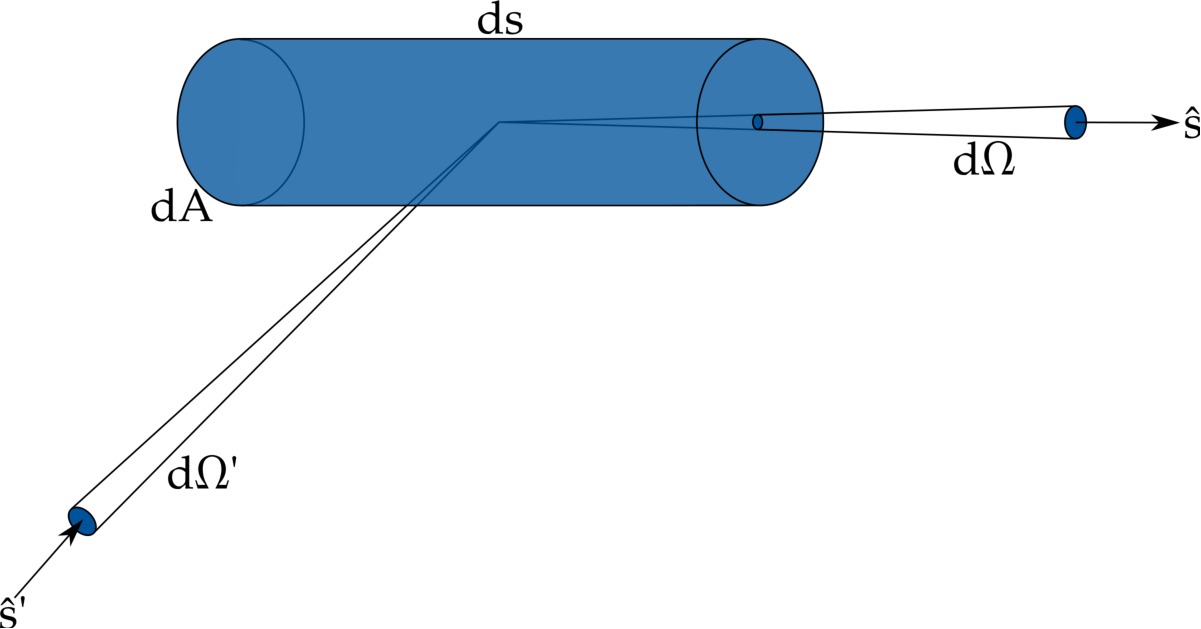
\includegraphics[scale=0.75]{cylinderelement.pdf}
	\caption{Cylindrical volume element, $ds \cdot dA$, with solid angle $d\Omega$ in direction $\hat{s}$ and solid angle $d\Omega'$ in direction $\hat{s}'$. Energy flowing through this element is used to derive the \gls{rte}. Adapted from~\cite{wang2012biomedical,chandrasekhar2013radiative}.}
	\label{fig:energydiag2}
\end{figure}

In general, the \gls{rte} is hard to solve in arbitrary 3D geometries, however there are a number of approximations, and numerical methods available. Diffusion approximation, \gls{km}, and \gls{mcrt} are the common methods used to approximate the \gls{rte}.

\paragraph{Kubelka-Munk theory}
\gls{km} was originally developed in order to calculate the light distribution in thin layered materials, such as paint or paper~\cite{barbaric2011kubelka}. The theory is rather simple and makes many assumptions about the medium and the incident light. The main assumptions of \gls{km} are: only scattering and absorption take pace in the medium, the incident light is already diffuse, the medium is uniform, only isotropic scattering, no external or internal reflections, and the medium is planar and infinitely wide~\cite{jasinski2011modelling,cheong1990review,gabriela2013mathematical}.

These assumptions make \gls{km}, very poor for modelling light-tissue interactions. This is as in tissue, scattering is not isotropic, but rather forward biased (see~\cref{sec:optprop}). Tissue is rarely, if ever, planar and infinitely wide. Tissue also has some reflections at its external and internal boundaries, due to change in refractive indices. Many medical and biophotonic treatments/methods use laser light which is not diffuse. Finally tissue can also exhibit fluorescence, which \gls{km} is not able to model, along with polarization. 
\Gls{km} does have some positive aspects. It is good at calculating the diffuse reflectance of simple mediums, and can be used to roughly estimate calculations. Though it is not well suited for modelling light-tissue applications.***refs for these claims***

\paragraph{Diffusion approximation}
The diffusion approximation for the \gls{rte}, is where the irradiance is separated into two components:

\begin{equation}
	L(\vec{r},\hat{s}) = L_c(\vec{r},\hat{s}) +l_d(\vec{r},\hat{s})
\end{equation}
Where $L_c$ is the unscattered contribution, which satisfies Beer's law\footnote{Beer's law (or Beer-Lambert law) states that the transmission, $T$, is equal to $e^{-\mu L}$, where $L$ is the distance and $\mu$ is the attenuation coefficient.}, and $L_d$ is the diffuse contribution. The $L_d$ component is expanded using Legendre polynomials and truncated. 
The diffusion approximation also has a number of assumptions and restrictions. The main assumption is that scattering dominates over absorption, and that the scattering is nearly isotropic. This restricts the types of scattering the Diffusion approximation can model, though using similarity relations can partially model scattering in tissue~\cite{graaff1993similarity,yoon1989accuracies}.

Diffusion theory is computationally fast, and simple. However it is poor at modelling light-tissue interactions due to it's assumptions and restrictions, mainly the inaccurate modelling near the boundaries of the medium and its lack of modelling fluorescence and other microphysics. However it can be used to speed up \gls{mcrt} in optically thick regions~\cite{robitaille2010modified,min2009radiative}.

\medskip

The final method, \gls{mcrt}, is a method that is numerically equivalent to the \gls{rte}~\cite{wang2012biomedical}. \Gls{mcrt} is a very flexible method, it can model arbitrary 3D geometries, various microphysics: fluorescence, and polarisation. It can also model various different light sources, from collimated laser beams, to diffuse light sources. The only downside that is noted in the literature is that the \gls{mcrt} can be very expensive computationally. However with computational power growing faster with each year, this is less and less of a problem going forward. The next several sections give an in depth description of the \gls{mcrt} method and it's flexibility, along with a description of the code used in this thesis to solve various medical and biophotonic problems.

\subsection{MCRT algorithm}

The \gls{mcrt} algorithm can be as simple as a $\sim$ 20 line program to as complex as needed for the problem at hand. This section will provide an in depth description of the \gls{mcrt} algorithm. The following section will provide details of how the \gls{mcrt} algorithm is implemented in the Fortran programming language, along with the various code details, such as the implementation of the 3D voxelised medium.



%***this section will be transformed into basic MCRT algo section. The following section will %describe the code in detail.***
%
%steps
%
%set up medium
%setup init pos & dir -> derivation of dir vectors -> mention
%get tau -> normalise 
%move photon
%scatter
%repeat
%
%code shizz
%
%voxel medium - gridset
%transport in grid tauint
%sourceph
%scatter -> derivation of non lab frame shizz stokes
%absorb
%path length estimators
%write out data
%
%overall structure

\subsubsection{medium set-up}\label{sec:algomedium}
The first step of any \gls{mcrt} algorithm , is to set-up the medium the photons will propagate through. There are a variety of ways that the medium can be set-up, for this section, we will assume the medium is an isotropic sphere, radius R, and centred at the origin. for simplicity we will only consider one wavelength, $\lambda$. The following section will detail arbitrary geometries and cases where there are more than one wavelength of interest.


\begin{figure}[!ht]
\centering
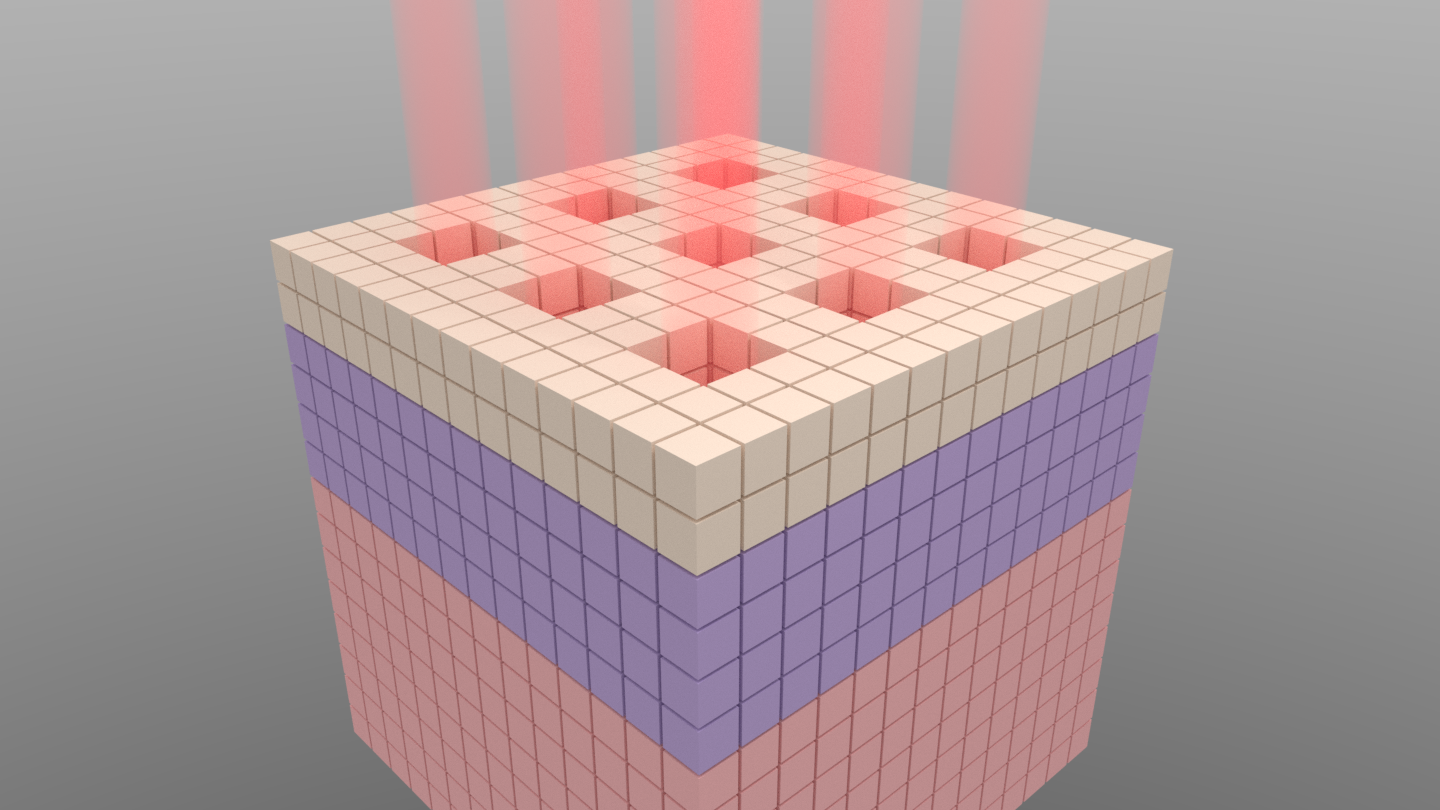
\includegraphics[scale=0.25]{voxel-model-render.png}
\caption{Example of a possible voxel model, with three different layers, various holes due to ablative pixel beam lasers. Each voxel can represent a different optical/thermal propertty of the tissue medium.***move to correct place***}
\label{fig:voxel-model}
\end{figure}

\subsubsection{Grid set-up}\label{sec:photsetup}

The first step of the \gls{mcrt} algorithm is to set-up the grid which acts as the simulated medium. This grid consists of $n \times n \times n$ voxels\footnote{A voxel is a 3D pixel} of which each voxel has it's own optical properties~(see \cref{sec:optprop} for discussion). This allows the medium of interest to be discretised onto a grid, which gives a good approximation of the real-life medium (see~\cref{sec:codefurther} for discussion on this). along with setting up the medium, arrays which store the locations of the voxel walls in each cardinal direction are created for reference in later parts of the code. Once the medium has been set-up photon packets are launched and propagated through the voxel structure.


\subsubsection{Photon launch}\label{sec:photlaunch}

The initial step (besides medium set-up and other book keeping) of any \gls{mcrt} algorithm is to launch a photon packet. Depending on the source of photon packets for a given simulation, this step varies from simulation to simulation. The general idea of launching a photon packet is that the packet is given an initial direction vector and position (which consists of a physical position and a voxel position)\footnote{all variables given in this section are the same as they are in the code.}:

\begin{align}
	direction &= \begin{bmatrix}
		n_{xp}\\
		n_{yp}\\
		n_{zp}
	\end{bmatrix}\\
	position &= \begin{bmatrix}
		x_p, y_p, z_p\\
	\end{bmatrix}\\
	voxel &= \begin{bmatrix}
		x_{cell}, y_{cell}, z_{cell}
	\end{bmatrix}	 
\end{align}

In order to set the direction vectors, the components of the direction vectors must be first set. The packets position is tracked using a Cartesian coordinate system, however for ease of computation for calculating scattering angles (see~\cref{sec:photscatterabsorb}), the direction vectors are computed in a spherical system thus the direction vectors are: 

\begin{align}
n_{xp} &= sin(\theta) \cdot cos(\phi) \\
n_{yp} &= sin(\theta) \cdot sin(\phi) \\
n_{zp} &= cos(\theta)
\end{align}

$\theta$ and $\phi$ are generated dependant on the photon source used. The individual sine and cosine terms are saved for use in the scattering routines, see~\cref{sec:photscatterabsorb}.

\subsubsection{Photon move}\label{sec:photmove}

The next step in the algorithm is moving a packet to the next interaction point. The probability a packet will interact over a distance $dL$ is $\mu_tdL$, where $\mu_t$ is the interaction probability (see~\cref{sec:optprop}). Thus the probability of travelling $dL$ without any interaction is $1-\mu_tdL$. Therefore over a distance $L$, with N segments of length $L/N$ the probability of travelling $L$ before any interaction:

\begin{align}
P(L) &= (1-\mu_t\frac{L}{N}) \cdot (1-\mu_t\frac{L}{N}) ...\ (1-\mu_t\frac{L}{N}) = (1-\mu_t\frac{L}{N})^N \\
P(L) &= \lim_{N \to \infty}(1-\mu_t\frac{L}{N})^N=e^{-\mu_tL}=e^{-\tau}\label{eqn:pdfdist}
\end{align}

Where $\tau$ is the number of mean free paths over a distance L. We now have a \gls{pdf}, \cref{eqn:pdfdist}, for the distance a packet will travel before an interaction occurs. For this to be of use we need to be able to sample from this \gls{pdf} in order to get a random optical depth. Using the Monte Carlo method described in~\cref{sec:mcmethod}, with $\xi$ as our random variable, we get:

\begin{equation}
\xi=\int_{0}^{\tau}e^{-\tau'}=1-e^{-\tau}\rightarrow \tau=-log(1-\xi)
\end{equation}

As $\xi$ is symmetric about 0.5 we can substitute $1-\xi$ for $\xi$ yielding:

\begin{equation}
\tau=-log(\xi)\label{eqn:taueqn}
\end{equation} 

We now have an optical distance, however we need to convert this into a physical distance so that we can move our photon packet. From our definition of $\tau$ we know that $\tau=\int_0^L\mu_tdS$, and if we have a smooth, homogeneous medium (i.e not a gridded medium) thus 

\begin{equation}
L=\frac{\tau}{\mu_t}\label{eqn:physicaldist}
\end{equation}

Therefore in order to update the packets position is simply:

\begin{align}
x_p &= x_p+L\cdot n_{xp}\label{eqn:update1}\\
y_p &= y_p+L\cdot n_{yp}\label{eqn:update2}\\
z_p &= z_p+L\cdot n_{zp}\label{eqn:update3}
\end{align}

However as the code in this thesis is a 3D gridded Cartesian code, we have to slightly adjust how we move and update the packets position. As stated in~\cref{sec:photsetup}, the medium has been discretised onto a grid, so that each voxel can have a different $\mu_t$, thus~\cref{eqn:physicaldist} becomes:

\begin{equation}
L=\frac{\tau}{\mu_{t,\zeta}}\quad\quad \zeta=(x,y,z)
\end{equation}

with $\mu_{t,\zeta}$ the $\mu_t$ for the $\zeta^{th}$ voxel. The position is then updated as before using~\cref{eqn:update1,eqn:update2,eqn:update3}. The next step in the algorithm is the interaction event, which can consist of either: scattering, absorbing or fluorescing.

\subsubsection{Photon scatter and absorbing}\label{sec:photscatterabsorb}

The first part of this section of the algorithm is to decide what kind of interaction the packet has with the medium. This section will focus on scattering and absorbing with other interaction events left for the chapters that detail these behaviours.
\medskip

To decide whether a packet scatters or absorbs involves `throwing' a random number and comparing it against the albedo. As detailed in~\cref{sec:optprop} the albedo is the scattering probability $a=\tfrac{\mu_a}{\mu_a+\mu_s}$. The random number is compared to the albedo, and if the random number is less than the albedo then the packet scatters, otherwise the packet is absorbed.

\paragraph{Packet absorption}\hspace{0pt}\\
\\
If the interaction event is a photon packet absorption, then the algorithm terminates the photon packets and starts the next photon packet,~\cref{sec:terminator}.

\paragraph{Packet scattering}\hspace{0pt}\\
\\
If the interaction event is a packet scattering, then the packet is scattered into a new direction and the above process are carried out until a termination clause is met, see~\cref{sec:terminator}.

Depending of the medium being simulated, it can either be isotropically scattering or preferentially scattering in a direction. In the case of simulating photon propagation in tissue, tissue is highly forward scattering.

Anisotropy is the degree of deviation in the photon packets path at each interaction event. The measure of anisotropy is the g value, $g$. With $g$ taking any value from $-1$ to $1$, $-1$ is highly backward scattering, $0$ is isotropic scattering and $1$ is highly forward scattering. 


\subsubsection{Termination}\label{sec:terminator}

\subsection{Code details}

This section details the the actual implementation of the \gls{mcrt} algorithm detailed in the previous section, along with any computational necessities and speed ups on the original algorithm.

\section{Validation of MCRT code}
\section{Optical properties}\label{sec:optprop}

Optical properties of a medium are the properties that determine how light is transported though that medium. Usually the optical properties of a medium are defined by three main parameters: the scattering and absorption coefficients ($\mu_s$ and $\mu_a$), and the anisotropy coefficient ($g$). There are several other optical properties the medium can be defined with, however these in general are only used for specific applications, such as Raman cross-sections for Raman scattering.

\subsection{Scattering}\label{sec:scatt}

The scattering coefficient, along with the anisotropy value (see ~\cref{sec:ansio}), define how light is scattered in a medium. Scattering occurs in skin due to a number of different scatterers, and inhomogeneities found within the skin. The main scatters in the skin are filamentous proteins such as collagen and elastin. These proteins are generally found within the dermis and epidermis~\cite{jacques1996origins}. In the upper layers of the skin, the main scatters are keratins and various chromophores such as melanin. 
The size of the aforementioned scatters affect how light is scattered and into which direction that light is scattered into.

\medskip

The scattering of light within tissue is usually defined as $\mu_s$ or $\mu_s'$: the scattering coefficient and the reduced scattering coefficient, where $\mu_s'=\mu_s(1-g)$. The scattering coefficient is defined such that the probability of transmission without scattering in a path length L is:

\begin{equation}
	T=e^{-\mu_sL}
\end{equation}
This gives units of inverse length for the scattering coefficient (usually measured in $cm^{-1}$). The reduced scattering coefficient is quite often given in place of the scattering coefficient, as the reduced coefficient is more easily measured then the `normal' coefficient~\cite{jacques2013optical}.



\subsection{Anisotropy}\label{sec:ansio}

Anisotropy is the degree of deviation that light undergoes at each scattering event. The anisotropy value is taken from the phase function for the medium. The phase function, $\Phi(\theta,\phi)$, is usually normalised over all angles:

\begin{equation}
	\int_{\Omega}\Phi(\theta,\phi)\ d\Omega = 1
\end{equation}

Where $\theta$, and $\phi$ are the usual spherical angles.
Thus the usual Rayleigh scattering and isotropic scattering, phases function's are:

\begin{align}
	\Phi_{isotropic}(\theta,\phi)&=\frac{1}{4\pi}\\
	\Phi_{Rayleigh}(\theta,\phi)&=\frac{3}{8\pi}(1+cos^2(\theta))
\end{align}

For simplicity, the phase function is usually cast as the anisotropy value g, which is defined as the average angle of deflection:

\begin{equation}
	g=\left<cos(\theta)\right>=\int_{\Omega}cos(\theta)\Phi(\theta,\phi)\ d\Omega
\end{equation}
The anisotropy factor, g, can take on any value from $-1$ to $1$. Where a value of $-1$ is highly back scattering, $0$ is isotopic scattering, and $1$ is highly forward scattering.


There are many phase functions that can be used to model the anisotropy factor in a medium. the standard phase function in biological tissue is the Henyey-Greenstein phase function. The Henyey-Greenstein phase function, was originally created to modelling diffuse radiation in the galaxy~\cite{lister2012optical,henyey1941diffuse}. The Henyey-Greenstein phase function has become the \textit{de-facto} phase function for biological tissue. This is due to the phase functions, relative simplicity and due to it being regarded as a `good' phase function for accurately modelling scattering in biological tissue~\cite{jacques1987angular}.
The Henyey-Greenstein phase function is shown in~\cref{eqn:henyey}:

\begin{equation}
	\Phi_{H.G}(\theta,\phi)=\frac{1}{4\pi}\frac{1-g^2}{(1+g^2-2g\ cos(\theta))^{\tfrac{3}{2}}}
	\label{eqn:henyey}
\end{equation}

\begin{figure}
	\centering
	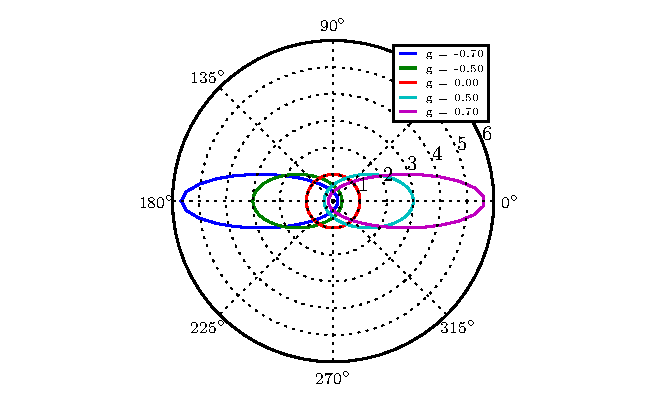
\includegraphics[width=\columnwidth]{polar.pdf}
	\caption{Figure show the g factor for the Henyey-Greenstein phase function, for various configurations of back, forward or isotropic scattering.}
	\label{fig:henyey}
\end{figure}

\subsection{Absorption}\label{sec:absor}

Absorption of light by a medium is defined by the absorption coefficient $\mu_a$. The absorption coefficient is defined, as before with the scattering coefficient, by considering the probability of transmission without absorbing in a path length L:

\begin{equation}
	T=e^{-\mu_aL}
\end{equation}
This, again like the scattering coefficient, gives inverse distance for the unit of the absorption coefficient (and its is also usually measured in units of $cm^{-1}$).

There are various sources of absorbers in tissue: blood, water, fat, melanin, $\beta$-carotene, bilirubin are among the more absorbing chromophores. These chromophores can all contribute, depending on the probing wavelength, with some more absorbing than others, see~\cref{fig:absorb}. 

\begin{figure}
	\centering
	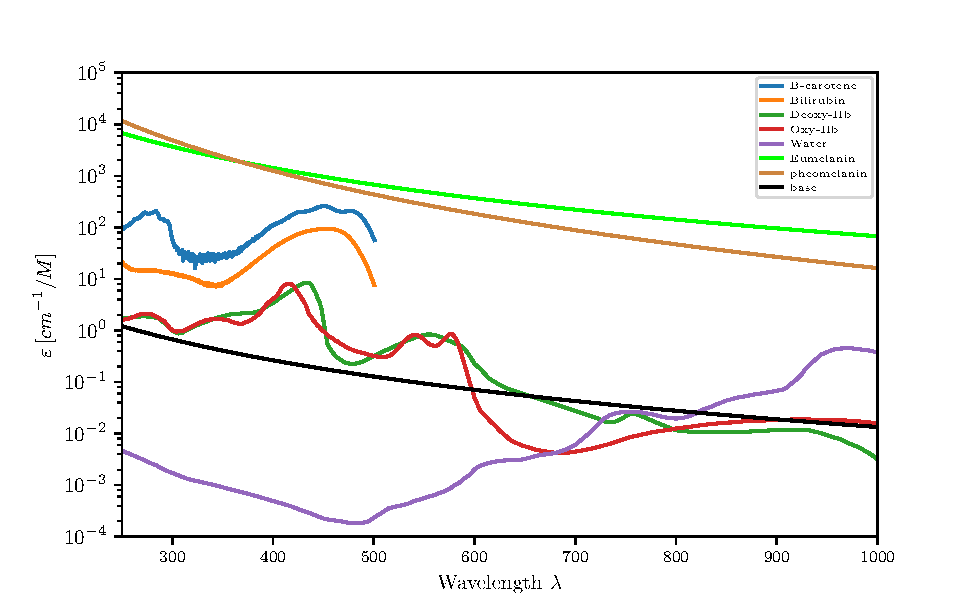
\includegraphics[width=\columnwidth]{absorbers.pdf}
	\caption{Spectra of some of the more common absorbers found in the skin~\cite{dixon2005photochemcad,photoprahl2017,segelstein1981complex,pope1997absorption,jacques2013optical,van2004determination,saidi1992transcutaneous,iglesias2015biophysically,bashkatov2011optical,sarna2006physical}.}
	\label{fig:absorb}
\end{figure}


\subsection{Other parameters}\label{sec:other}
The preceding subsection, described the optical properties that this thesis will use in every chapter. However there are other optical properties that can be used to define a medium. These other parameters generally are used to model microphysics such as Raman scattering, polarization, fluorescence or reflection/refraction. This section will give a brief overview of these other optical properties.

\medskip

\paragraph*{Refractive index}
The refractive index of a medium, defines how fast light propagates through that medium. Generally for tissue, the refractive index is given as a bulk refractive index. Meaning that the medium is divided into sections, with each section given a refractive index. For example, skin's refractive indices are divided up by the different layers of skin (as shown in~\cref{tab:refrac}).

\begin{table}[hb!]
	\centering

	\begin{tabular}{|l|cc|}
	\hline

	\hline
	\textbf{Layer} & \textbf{Refractive index} &\\
	\hline

	\hline
		Stratum Corenum & 1.53 & \\
	\hline
		Epidermis & 1.34 & \\
	\hline
		Papillary Dermis & 1.395 &\\
	\hline
		Reticular Dermis & 1.39 &\\
	\hline
		Hypodermis & 1.44 &\\
	\hline

	\hline
	\end{tabular}
	\caption{Example of refractive indices per layer of skin for a $\lambda$=632.8~nm~\cite{meglinski2002quantitative}.}
	\label{tab:refrac}
\end{table}

Details on how refraction is implemented with the code can  be found in ***ref here***.

\medskip

\paragraph*{Raman Scattering}
Raman scattering is where a photon is scattered inelastically, which excites the molecule the photon scattered off, thus decreasing the energy of the photon and increasing the photons wavelength. The optical property needed to model Raman scattering, is the Raman scattering cross section. The cross section, like the absorption or scattering coefficient, is the likelihood of a photon undergoing a Raman scattering event. Raman scattering has been modelled in \gls{mcrt} in order to simulate spatially offset Raman spectroscopy for breast tumour analysis~\cite{keller2010monte}.

\medskip

\paragraph*{Fluorescence}
Fluorescence occurs when a photon is absorbed by a fluorescent molecule and re-emitted with a new wavelength. Fluorescence	is a reactively common phenomena, and is heavily utilised in biophotonics and medicine, in order to image, or monitor molecules in tissue. Again the optical property that models fluorescence is coefficient that gives the probability of absorption and re-emission of a photon by a certain molecule. Usually this is in the form of an absorption coefficient or extinction coefficient. The extinction coefficient is a measurement of absorption in terms of the concentration of that absorber. Thus if a medium has many fluorophores, then the total absorption coefficient is the bulk absorption of the medium plus the contribution from the fluorophores as in~\cref{eqn:exct}:

\begin{equation}
\mu_a=ln10 \sum_i C_i \varepsilon_i
\label{eqn:exct}	
\end{equation}

Fluorescence will be described in more depth in~\cref{sec:salvo,sec:madrid}.

\section{Further extensions to the code}\label{sec:codefurther}
This section details the miscellaneous additions to the \gls{mcrt} algorithm that the various chapters in this thesis may or may not use.

\subsection{Fresnel reflections \texorpdfstring{$\&$}{and} refractions}\label{sec:fresnel}
***this section in madrid work?***


\begin{align}
	R_s&=\left|\frac{n_1\ cos\theta_i-n_2\ cos\theta_t}{n_1\ cos\theta_i+n_2\ cos\theta_t}\right|^2\\
	R_p&=\left|\frac{n_1\ cos\theta_t-n_2\ cos\theta_i}{n_1\ cos\theta_t+n_2\ cos\theta_i}\right|^2
\end{align}

\subsection{Parallelisation of the \texorpdfstring{\gls{mcrt}}{MCRT} algorithm}\label{sec:parasec}

As mentioned in the previous sections, \gls{mcrt} can be computationally intensive, especially when dealing with highly scattering mediums. Fluorescence can also cause simulations times to drastically increase as photons are no longer `killed' off, but rather re-emitted at a new wavelength. Other optical processes such as Raman scattering are highly unlikely events, which again can lead to a dramatic increase in simulation times, as many photons are required to be simulate in order to get `good' statistics.

Fortunately \gls{mcrt} is classed as an `embarrassingly parallel' problem\footnote{However this is not true for all \gls{mcrt} applications. For example using the Bjorkman $\&$ Wood~\cite{bjorkman2001radiative} immediate temperature corrections method, turns \gls{mcrt} into a different class of parallel problem~\cite{robitaille2011hyperion}.}. This means that it is trivial to parallelise in comparison to other algorithms. The reason that \gls{mcrt} is classed as `embarrassingly parallel', is that the algorithm can be split up onto separate processes, with no little need for communication between them. In reality this means that $n$ copies of the algorithm can run on $n$ cores in a processor, with communication taking place at the start and end of each simulation run. 

All the code in this thesis is parallelised using \gls{mpi}, with the only communication taking place at the end, where the path length estimators are collated on to all process. 

***ToDO***
do parallel tests
finish writing this subsection
***ToDO***

\section{Improving the voxel tissue model}\label{sec:improve}

***Needed?***

As voxels are cuboid in shape, in order for them to accurately model biological tissue, which is decidedly not smooth, new methods or approximations were attempted to improve the modelling of biological tissue. 
The first is bump-mapping, a technique borrowed from computer graphics. The second is to dispense with the voxel model and use a triangular based mesh. Both these methods were tried during the course of this thesis, but were abandoned due to time constraints. This section gives a brief overview of these techniques and why they were not ultimately used in this thesis.
